As explained in Section~\ref{sec:intro} OpenMP 4.0 / 4.5 provides two environment variables OMP\_PROC\_BIND and OMP\_PLACES to help users define the thread placement and bindings for their OpenMP application which we refer to as \textit{OpenMP Affinity}.%
%\begin{figure}[h!]
%  \centering
%  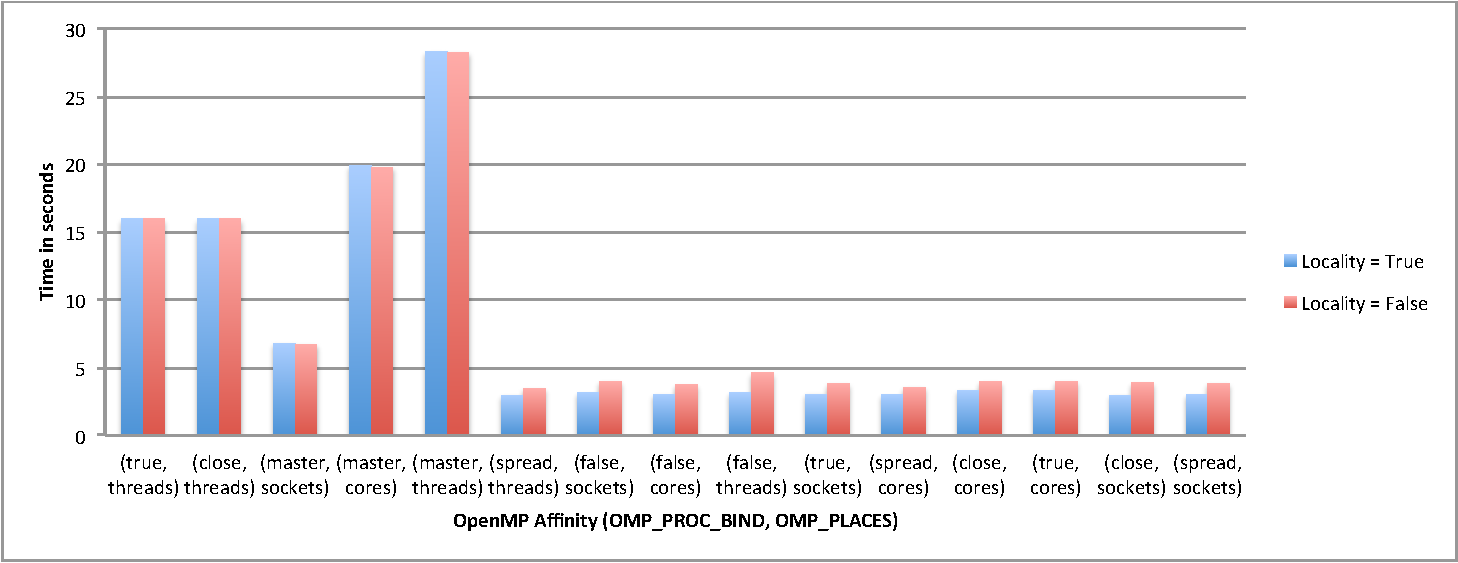
\includegraphics[height=0.4\textwidth, width=0.8\textwidth]{./Images/10Perf.pdf}
%       \caption{Performance with 10 OpenMP threads on \textit{}}
%       \label{fig:10th}
%\end{figure}
%
 We experiment with two version of the Jacobi program: a version that is optimized for data locality via correct memory placement using the first touch policy and another version where 
 all the data is close to where thread 0 is.   We use a jacobi problem size of (60000 X 60000)  to make to stress the memory subsystem, specifically to utilize the entire L3 and L4 caches.
 
 We run both programs with 10, 20, 40, 80 and 160  number of threads threads with different OpenMP affinity settings and record the POWER8 hardware counters.
 Figure~\ref{fig:20th} shows the performance of 20 OpenMP threads with different OpenMP Affinity settings. We observed that after 20 OpenMP threads the speedup does not vary significantly. The best speedup and efficiency combination (16 speedup, 80\% efficinecy) is achieved with 20 OpenMP threads with the OpenMP Affinity configuration of \textit{(spread, threads)}.
%
\begin{figure}[h!]
  \centering
  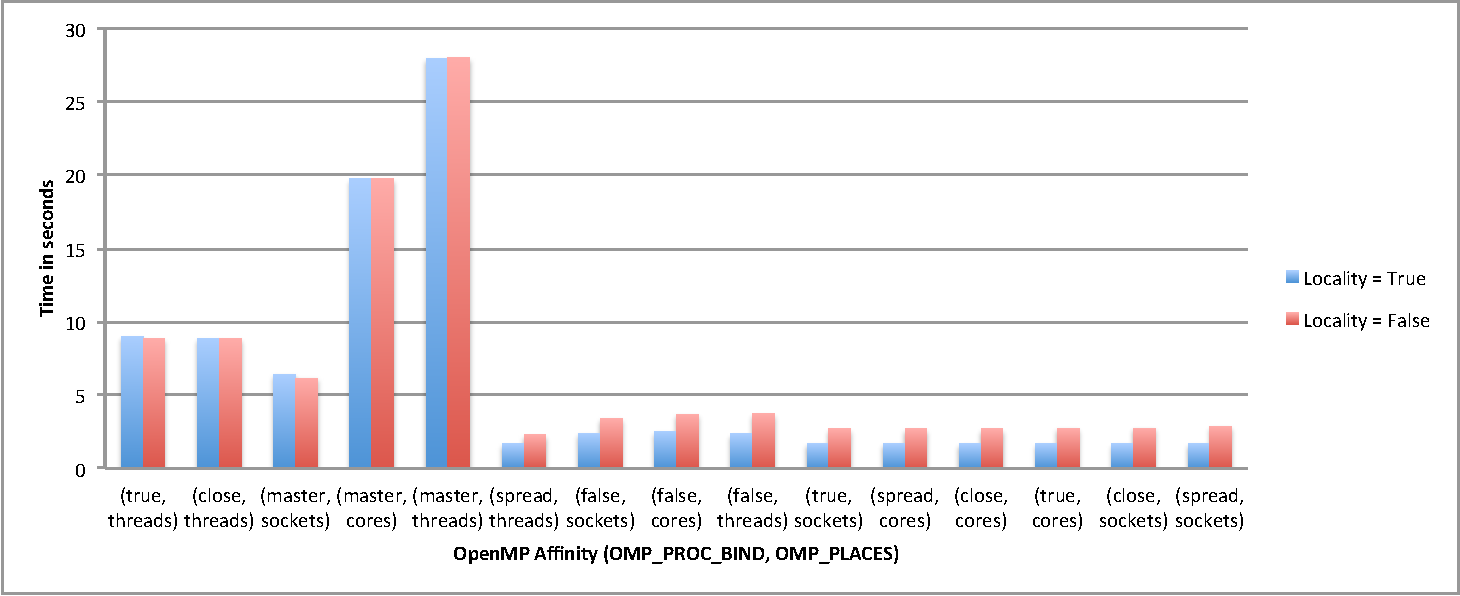
\includegraphics[height=0.4\textwidth, width=0.95\textwidth]{./Images/20Perf.pdf}
       \caption{Performance with 20 OpenMP threads on a two POWER8 socket system for the two versions of the Jacobi program.}
       \label{fig:20th}
\end{figure}
%
\begin{figure}[h!]
  \centering
  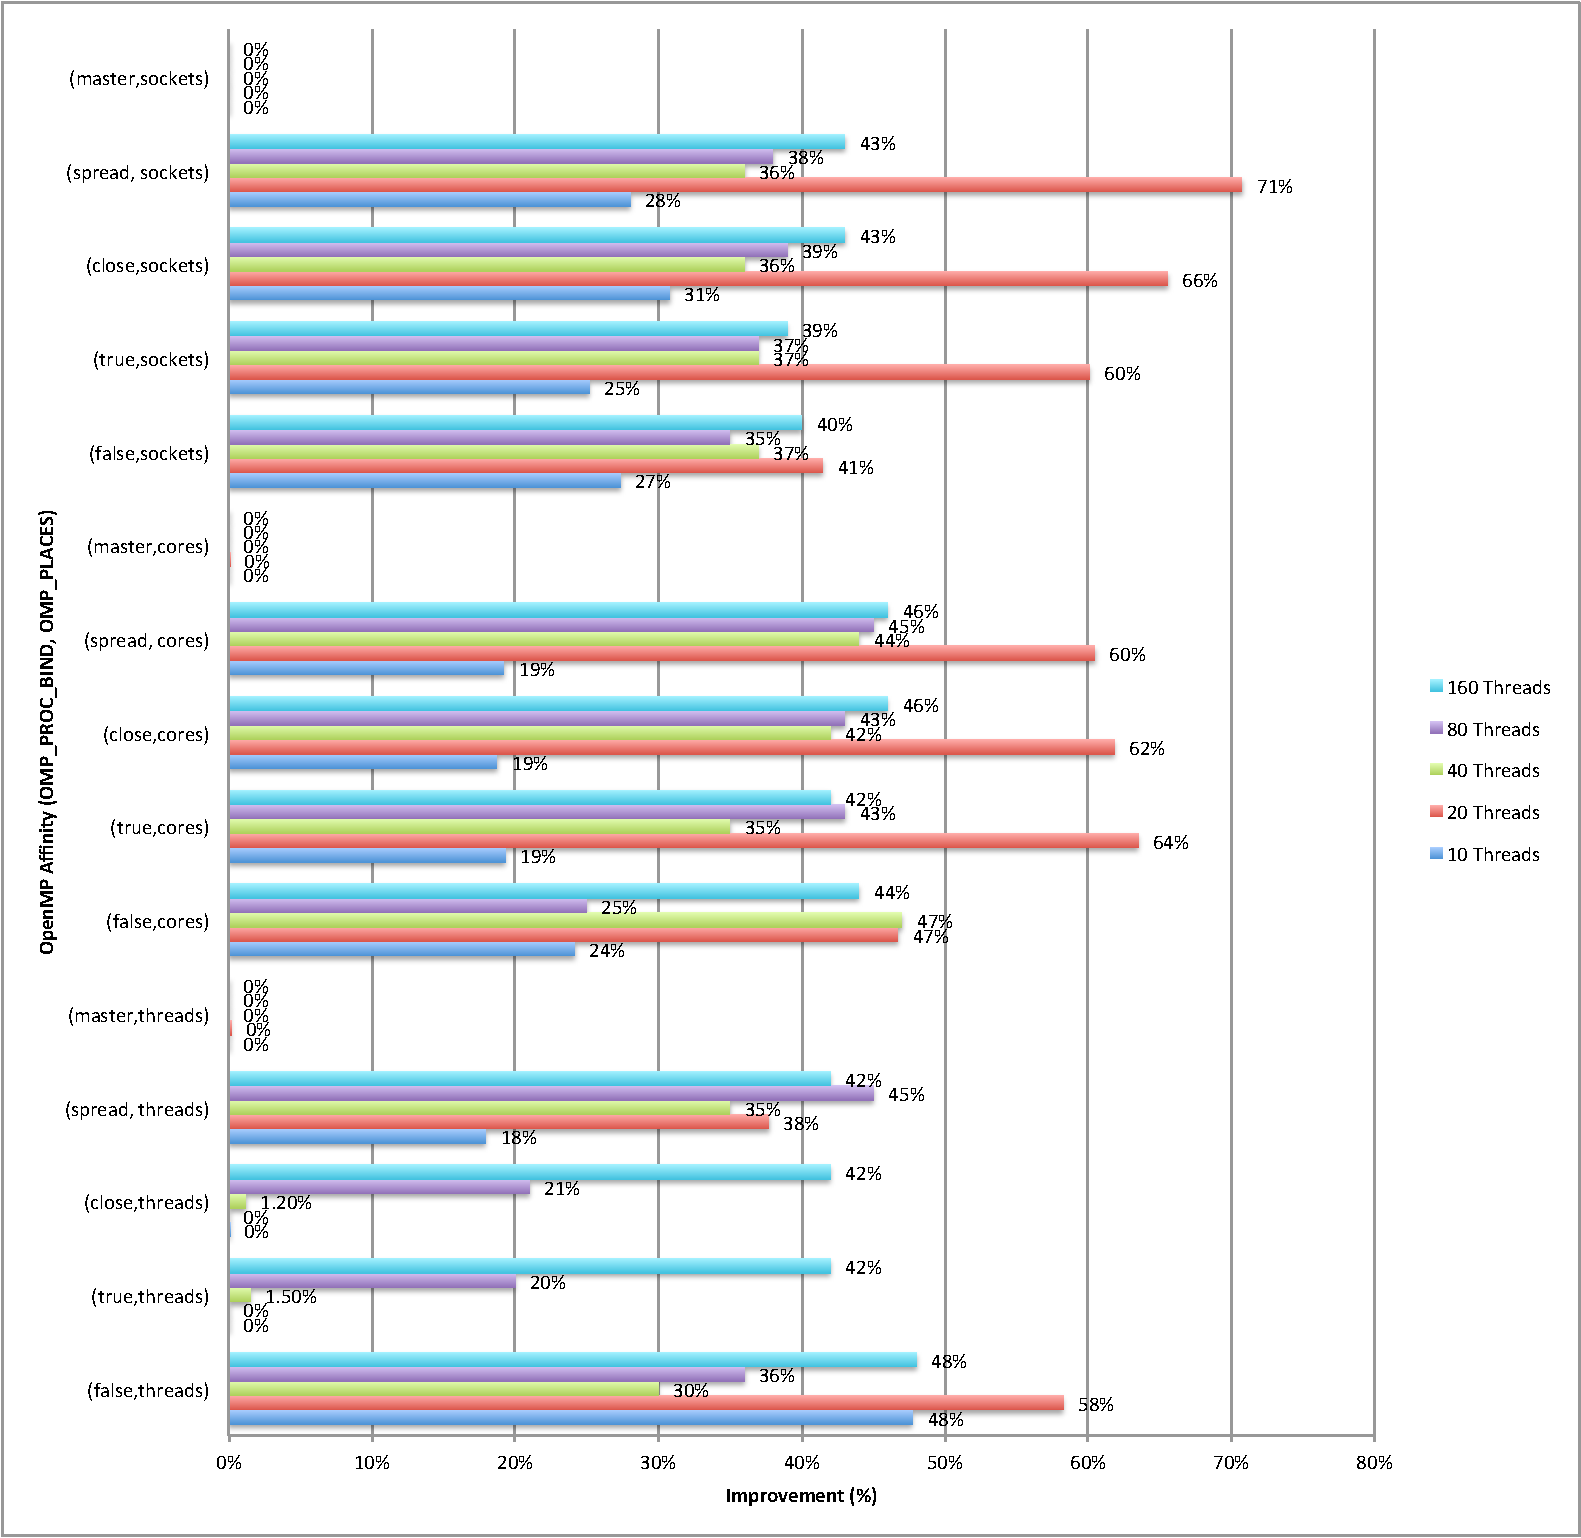
\includegraphics[height=1.4\textwidth, width=0.95\textwidth]{./Images/ImpAllV.pdf}
       \caption{Comparing Performance Improvement between the two version of the Jacobi program using 
       different number of OpenMP threads and thread affinity settings on a two POWER8 socket system}
       \label{fig:imp}
\end{figure}

Figure~\ref{fig:imp} shows the improvement of the locality-aware optimized version (with good data placement) of the Jacobi program over the unoptimized locality-unaware (all data local to thread 0) version when using different OpenMP Affinity settings for different OpenMP thread counts. 
We observe that for the \textit{(master, threads)} OpenMP affinity configuration all threads execute on a single hardware thread (CPUID 0).
 
When using \textit{(master, core)}, all threads execute on the different hardware threads that belong to the core where the master thread is running (the P8 processor has eight hardware threads per core), similarly for \textit{(master, socket)} all threads execute in the hardware threads of the socket where the master thread is running. In this case all threads will be bind to any of the CPU ids from 0 to 79. When OMP\_PROC\_BIND set to master we see in Figure ~\ref{fig:imp} that there is no improvement on the locality aware over the non-locality aware versions (e.g. using first-touch policy) because all the threads are running using the 
same NUMA domains. For \textit{(close, threads)}, we observe that all OpenMP threads run on hardware threads close to each other (on CPU ids: 0-19). 
All of these cases don't suffer from memory locality issues because they access memory memory that belong to the same NUMA domain or memory that is local to the socket (e.g. two NUMA domains per socket).
In the \textit{(spread, sockets)} and \textit{(close, sockets)} configuration threads are spread across sockets but may be mapped to hardware threads running on same core. We observed that the \textit{(true, threads)} configuration is equivalent to the \textit{(close,threads)} according to the GCC OpenMP runtime thread mappings.
For all OpenMP affinity settings  with OMP\_PROC\_BIND set to false, threads can migrate and are not bound to a specific thread, core or socket. This migration makes it less impactful on the data placement, but suffers from degraded performance.

From the above discussion it is clear that not all OpenMP Affinity configurations are equal, moreover currently it lacks the ability to specify affinity based on NUMA \textbf{and} NUCA domains of emerging architectures like POWER8. This is the first step in understanding the need for new OpenMP affinity features to successfully deploying OpenMP on POWER machines. %Need something more here. 
\begin{figure}[h!]
  \centering
  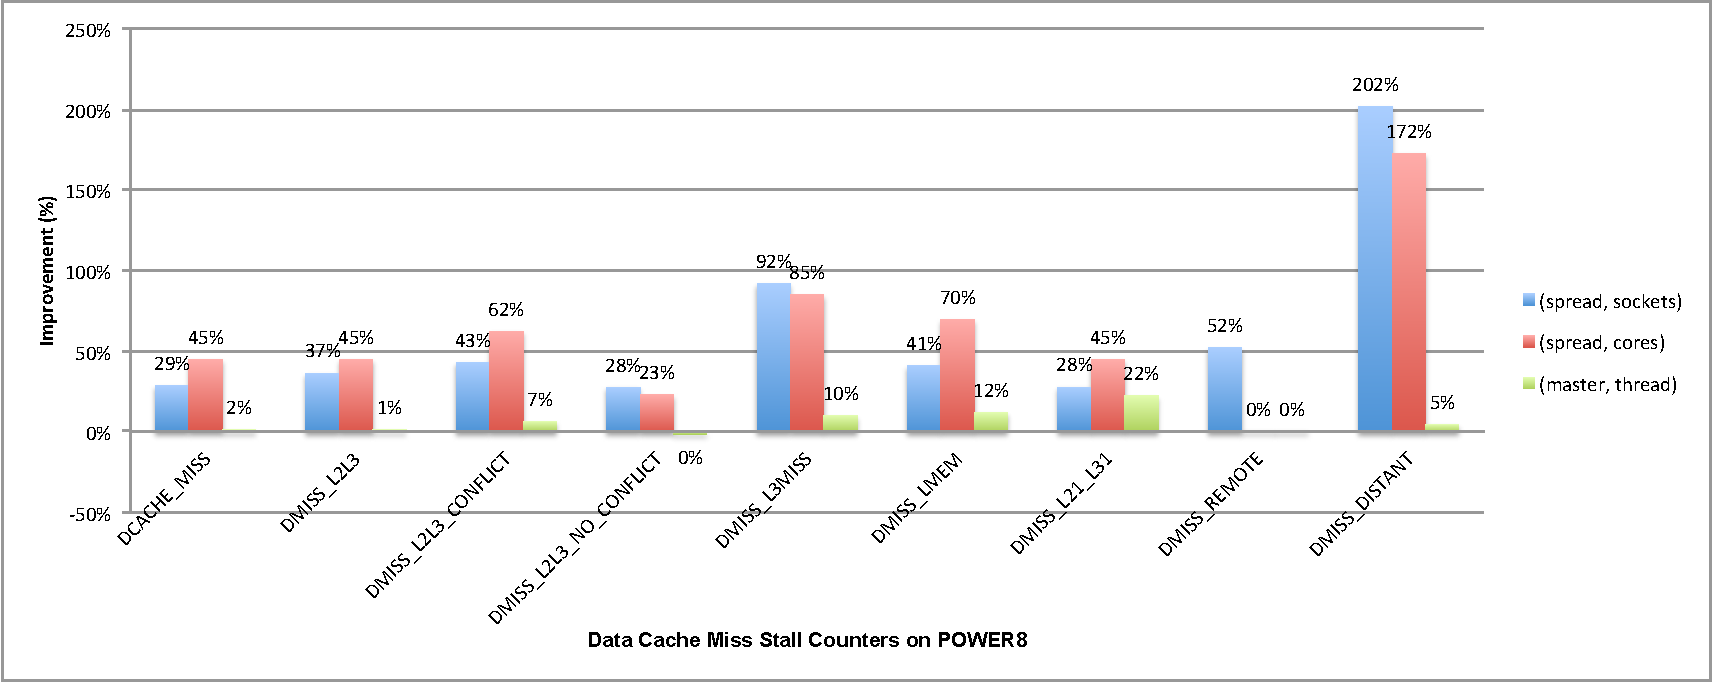
\includegraphics[height=0.4\textwidth, width=0.95\textwidth]{./Images/HW.pdf}
       \caption{Comparing Hardware Counter Change}
       \label{fig:HW}
\end{figure}
%
%Hardware Counter notes
Next we look at the hardware counters on the POWER8 system corresponding to the different configurations to explain the improvement we observed in Figure~\ref{fig:imp}.

%to see what hardware counters could potentially be used as indicators to signify a OpenMP Affinity choice for a given problem. 
We select the three cases of OpenMP Affinity tuple that represent the best, mid, and worst improvement as seen in Figure~\ref{fig:imp}. 
%the cases where we see more improvement for data locality on a given affinity setting 
Selected cases are \textit{(spread, sockets)},  \textit{(spread, cores)}, and \textit{(master, thread)}. 
For these cases we record the hardware counters for the locality aware and locality unaware versions and calculate the improvement as the value of their difference as a percentage of the value of the locality unaware hardware counter value. 
From Figure~\ref{fig:HW} we see that the two hardware counters that show the effects of data locality the most are DMISS\_DISTANT, DMISS\_L3MISS.
We would have expected to see more significant variation in the value of DMISS\_REMOTE, but we found that in some cases, these remote accesses can be cached.
For example, the case of \textit{(spread, sockets)} has better DMISS\_REMOTE improvement than  \textit{(spread, cores)} which is counterintuitive. 
This is because in \textit{(spread, sockets)} some threads (not all) are running on the same core sharing local cache lines for (L1, L2) and thus taking advantage of cache reuse for remote data access. 
This can also be seen by the significant improvement in DMISS\_DISTANT which quantifies the stalls by L1 reloads from distant interventions and memory. 

The improvements we see in \textit{(spread, cores)} are more due to DMISS\_L21\_L31, which shows a better utilization of the L2/L3 cache as this hardware counter measures the stall cycles by Dcache miss which are resolved on chip. 
In the case of  \textit{(spread, cores)} we are effectively increasing the amount of 
L2 cache available to each OpenMP thread, as each thread has access to its own L2 cache on a given core. 
For the \textit{(master, thread)} case, there is very little improvement in the memory subsystem utilization as everything is running on the same thread (or CPU id) and the most of the data is local to the socket. In this case the data-locality version does not make any difference because all the threads are time-sharing the same hardware thread. This is also true for the case  \textit{(close, threads)} where
 we don't see improvements on the data locality aware version since data is local to the threads. 
%%Option 1
%\begin{figure}[h!]
%  \centering
%  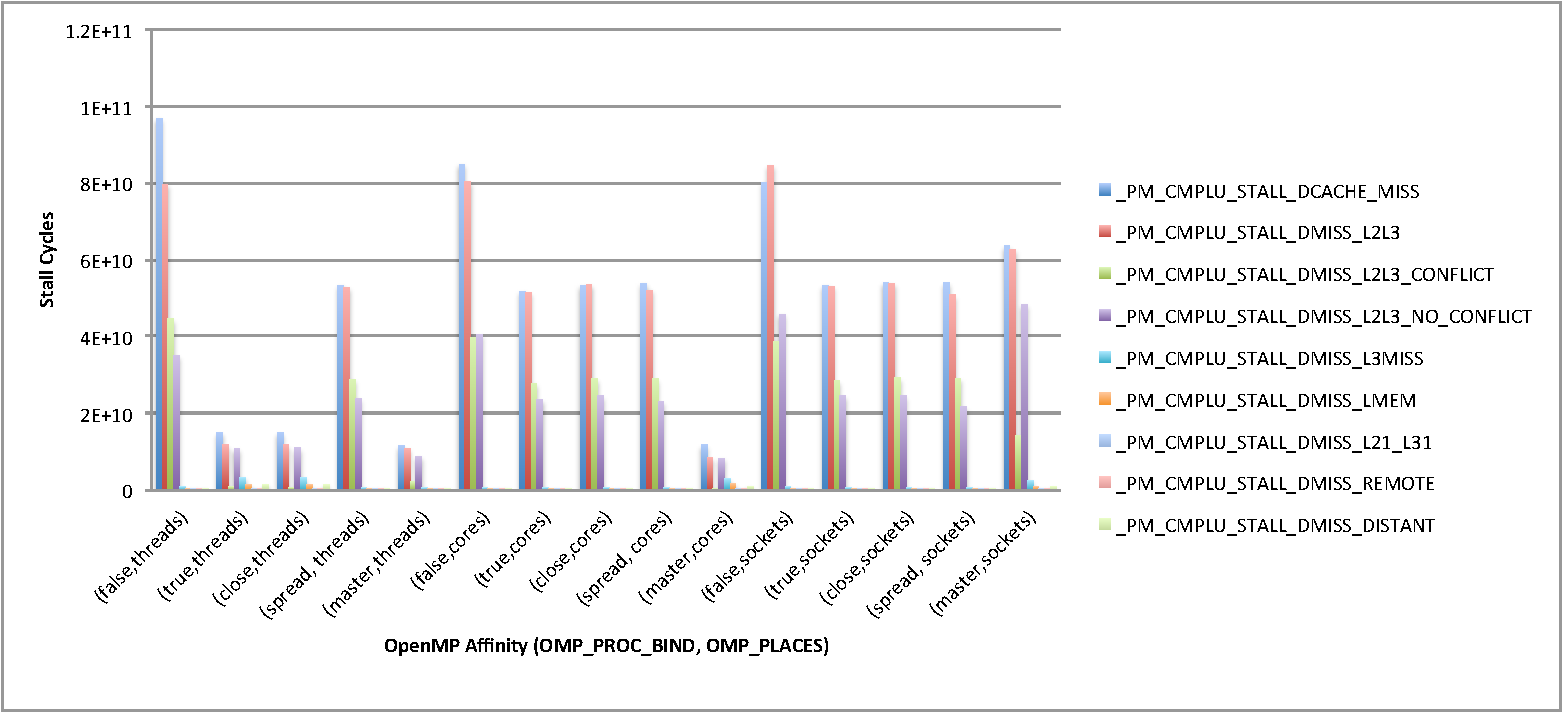
\includegraphics[height=0.4\textwidth, width=0.95\textwidth]{./Images/AllHW1.pdf}
%       \caption{Comparing Hardware Counters for Locality Aware Jacobi Program  Executions}
%       \label{fig:HW1}
%\end{figure}
%%Option 2
%\begin{figure}[h!]
%  \centering
%  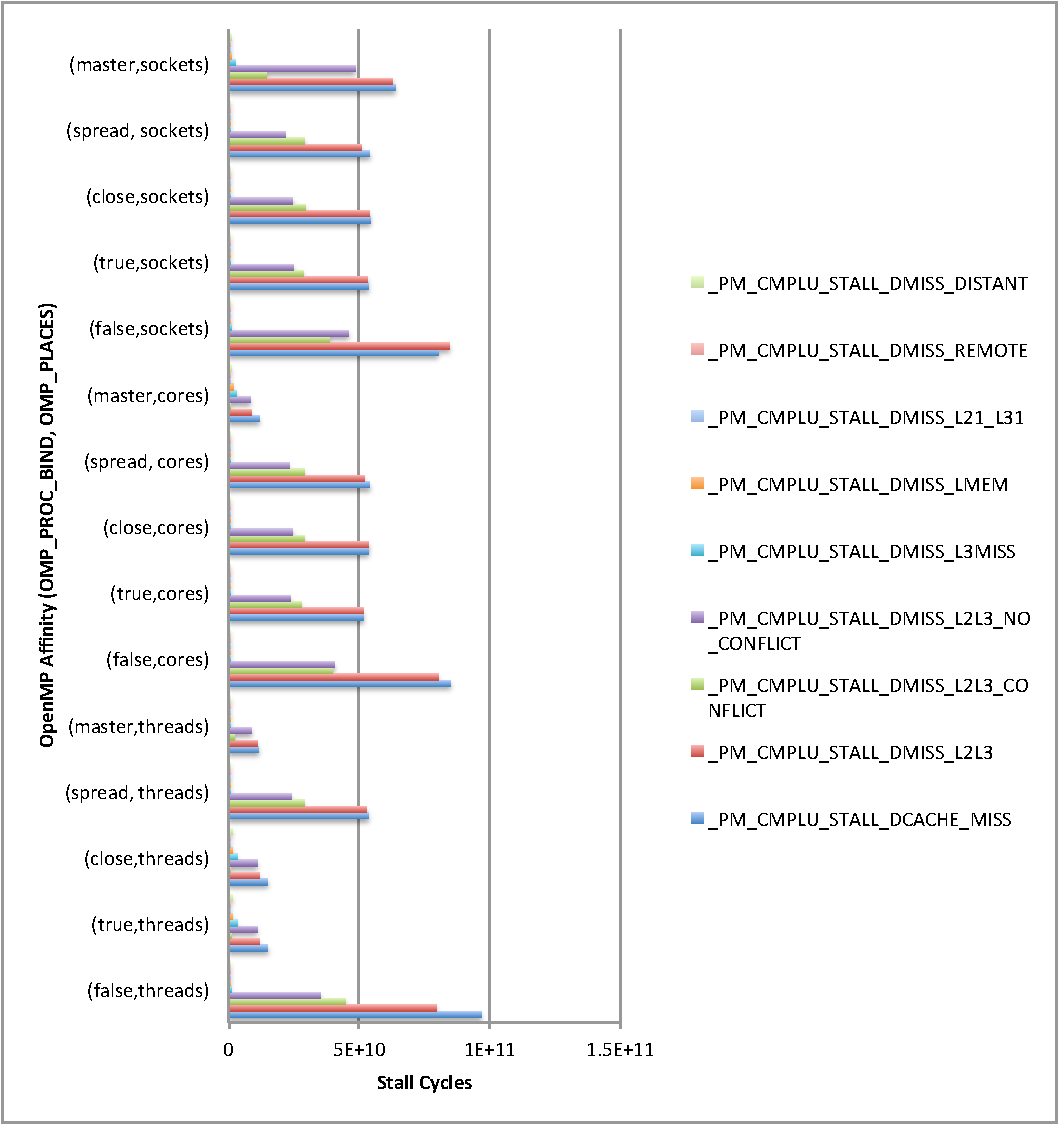
\includegraphics[height=1\textwidth, width=0.95\textwidth]{./Images/AllHW2.pdf}
%       \caption{Comparing Hardware Counters for Locality Aware Jacobi Program  Executions}
%       \label{fig:HW2}
%\end{figure}
%\begin{figure}[h!]
%  \centering
%  \includegraphics[height=0.4\textwidth, width=0.95\textwidth]{./Images/HW_RD.pdf}
%       \caption{Comparing Hardware Counters}
%       \label{fig:HW3}
%\end{figure}
%Figure~\ref{fig:HW3} shows the values of the stall cycles for the hardware counters discussed in Table~\ref{tab:hwct} and Table~\ref{tab:cl}. Though the individual values are not significant, the figure gives a clear idea of the relative difference in the hardware counter values for all locality aware runs. 

POWER8 provides these unique set of hardware counters to distinguish OpenMP configurations that have less useless cycles on the memory sub-system. Specifically, DMISS\_REMOTE and, more importantly, DMISS\_DISTANT are key in identifying if the program suffers from bad data locality as indicated in Figure~\ref{fig:imp}.
%For example, from the data collected for 20 OpenMP threads \textit{(spread, threads)},  \textit{(close, cores)}, \textit{(true, cores)},  \textit{(close, sockets)}, \textit{(spread, sockets)} have similar high speed-ups but the PM\_CMPLU\_STALL\_DMISS\_L2L3 is least in the \textit{(spread, sockets)} configuration. 


